\documentclass[12pt]{article}

% Language setting
\usepackage[utf8]{inputenc}
\usepackage[bulgarian]{babel}

% --------------------- Packages  --------------------
% Use biblatex
\usepackage{biblatex}
\addbibresource{bibliography.bib}
% Table thickness
\usepackage{ctable}
% Equations: SI units
\usepackage{siunitx}
% Approximately equal
\usepackage{amssymb}
% degrees symbol
\usepackage{gensymb}
% warning box
\usepackage{pifont,mdframed}

\newenvironment{warning}
  {\par\begin{mdframed}[linewidth=2pt, linecolor=white]%
    \begin{list}{}{\leftmargin=1cm
                   \labelwidth=\leftmargin}\item[\Large\ding{43}]}
  {\end{list}\end{mdframed}\par}

% --------------------- Title  --------------------
\addbibresource{bibliography.bib}
\title{Косвено измерване на обем на тяло}
\author{Виолета Кабаджова}
\date{October 2022}

\begin{document}

% Anfang der Titelseite________________________________________________________________________________
\begin{titlepage}
	\flushleft
% 	\begin{center}
	%{\scshape\Large Werkstoffe III \hspace{2.5cm} Laborbericht \hspace{2.5cm}HS 2022 \par}
	{\scshape\Large Протокол IV \hspace{2cm} Механика - практикум\par}
	\vspace{5cm}
	{\huge\bfseries Закон на Стокс\par}
	\vspace{1cm}
	{\LARGE\bfseries Лабораторно упражнение №16\par}
	\vspace{5cm}
    % {\LARGE\bfseries Физически Факлутет към Софийски Университет ``Св. Климент Охридски \par}
    {\LARGE\bfseries Виолета Кабаджова, \par}
%   {\LARGE\bfseries Group: X\par}
    {\large\bfseries ККТФ, фак. номер: 3PH0600026\par}
	\vspace{1cm}
	
	{\large Физически Факултет, 
	
	Софийски Университет "Св. Климент Охридски"
	
	9 ноември 2022 г.\par}
	
\end{titlepage}

\section{Теоритична част}\label{sec:theoretical-part}
\subsection{Сила на вътрешно триене според Нютон}
При реален флуид, движещ се ламинарно (без смесване на съседсните му слоеве), между тези слоеве възниква сила на вътрешно триене, чиято големина се определя от закона на Нюнон:
\begin{equation}\label{eq:newton-friction}
    F_{fr} = \eta \Bigg |  \frac{\Delta v}{\Delta x} \Bigg | \Delta S,
\end{equation}

където $F_{fr}$ - сила на триене\footnote{friction от английски}, $\eta$ е коефициент на вътрешно триене, $\Delta S$ - площта триещите се повърхности в направление, перпендикулярно на движението на флуида.
Важно е да се отбележи, че съпротивителната сила е резултат от триенетео между слоевете на течността, а не бива подбудена като резултат от нейното триене с тялото. Най-близкият до тялото слой бива "прилепнал" към него (т.е. се движи със скоростта на тялото), а скоростта на всеки следващ слой намалява с отдалечаване от тялото.

\subsection{Съпротивителна сила $F_c$}
Законът на Стокс за съпротивителна сила $F_c$, дейтстваща върху сфера, която извършва бавно и равномерно постъпателно движение в неограничена по обем течност, гласи:

\begin{equation}\label{eq:friction-force}
    F_c = 6\pi r \eta v,
\end{equation}

където $\eta$ - коефициент на вътрешно триене на течността, $v$ - скоростта на постъпателното двицение, a $r$ - радиусът на сферата. 

\begin{figure}
    \centering
    % 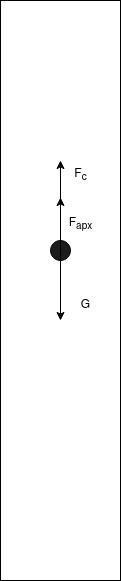
\includegraphics[width=0.1\textwidth]{images/Stocks_Equations.drawio.png}
    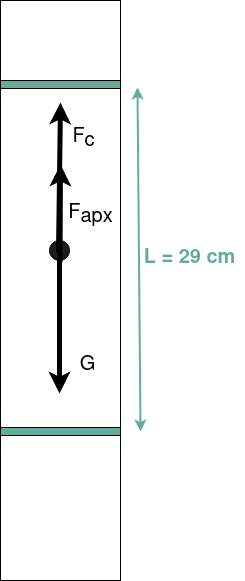
\includegraphics[width=0.2\textwidth]{images/Stocks_Equations_2.drawio.png}
    \caption{Илюстрация, показваща силите, действащи на тялото}
    \label{fig:forces}
\end{figure}

\subsection{Други сили, действащи на тялото}
Освен съпротивителната сила, описана в \ref{eq:friction-force}, върху тялото действат още сила на тежестта $G = m_{c\phi}g = \frac{4}{3}\pi r^3 \rho_{c\phi} g$, както и архимедова сила $F_{apx} = m_\tau g = \frac{4}{3}\pi r^3 \rho_{\tau} g$. Както се вижда от фиг. \ref{fig:forces}, силата на тежестта G е насочена надолу към цетъра на Земята, докато съпротивителната и архимедовата сила са насочени противопосочно. 

В началото на движението големината на силата на съпротивление малка поради зависимостта ѝ от скоростта на топчето, която също е малка. Следователно $G > F_{apx} + F_c$ и тялото се движи равноускорително до момент, в който силите се изравняват и тялото започва да се движи равномерно, в който момент $F_c = G$:

\begin{displaymath}
    6\pi r \eta v = \frac{4}{3} \pi r^3 (\rho_{c\phi} + \rho_{\tau})g,
\end{displaymath}

\begin{equation}\label{eq:eta}
    \eta = \frac{2}{9} \frac{\rho_{c\phi} + \rho_{\tau}}{v}gr^2
\end{equation}



\section{Експериментална част}
\subsection{Експериментална установка}\label{sec:experimental-setup}
Експерименталната установка е показана на фиг. \ref{fig:forces}. Няколко топчета, масата и диаметърът на всяко от които биват измерени непосредствено преди експеримента, биват пуснати едно след друго в тръба с дължина $l= 29cm = 0.29 m$ и с вътрешен радиус $R = 20.6 mm = 20.6 \cdot 10^{-3} m$. Тъй като формулата на Стокс, описана в \ref{sec:theoretical-part}. е в сила за тяло пуснато в неограничен флуид, а експеримента бива проведен в епруветка със стени и дъно, слагаме маркери в горната и долната част на епруветката, с които отбелязваме мястото, от което нататък считаме влиянието на ограничаването на флуида за пренебрежимо. Долният маркер служи за обозначаване на разстоянието от дъното на флуида, от което нататък влияението на дъното би било твърде значимо. Горният маркер служи за обозначаване на мястото, от което насетне трите сили, описани в \ref{sec:theoretical-part}., се уравновесяват.  

\subsection{Задача: Определяне коефициента на вътрешно триене на глицерин}
За целта следните подзадачи трябва да бъдат изпълнени за най-малко пет сфери:
\begin{enumerate}
    \item Определяне плътността по формулата $\rho_{c\phi} = \frac{m}{V} = \frac{m}{\frac{4}{3}\pi r^3}$;
    \item Определяне скоростта на сферата, когато тя започне да се движи равномерно (т.е. скоростта за времето, в което сферата се намира между двата маркера на фиг. \ref{fig:forces});
    \item Изчисляване на коефициента на вътрешно триене на течността по формула \ref{eq:eta}.
\end{enumerate}

След провеждане на експеримента от горепосочените стъпки създаваме таблица \ref{tab:meas} на база на различните видове топчета, които измерваме. Опит 1 е провден с един вид топче, опити 2 до 4 са проведени с друг, а опит 5 с трети.

\begin{table}[h]
\begin{center}
\begin{tabular}{|l|l|l|l|l|l|l|}\hline
N & m_i, [mg] &r_i, [mm] &t_i, [s] &\rho_i,[kg/m^3] &v_i, [m/s] & \eta_i, [Pa.s] \\ \hline
1 &64 &1.198 &16.03 &8886 &0.018 & 1.162 \\ \hline
\specialrule{.1em}{0em}{.2em}
2 &352 &2.175 &5.56 &8167 &0.052 & 1.092 \\ \hline
3 &349 &2.173 &5.58 &8120 &0.052 & 1.082\\ \hline
4 &347 &1.986 &5.5 &10576 &0.053 & 1.226\\ \hline
\specialrule{.1em}{0em}{.2em}
5 &359 &2.200 &4.79 &8049 &0.6 & 0.934\\ \hline
\end{tabular}
\end{center}
\caption{\label{tab:meas} Измервания от топчетата}
\end{table}

Имайки в предвид, че $\rho_{glycerin} = 1260.4 kg/m^3$ при 20 \degree C, $R = 20.6 \cdot 10^{-3} m$ и $l=29cm$. 
За да компенсираме грешката, получаваща се от ограничаването на флуида в даден обем, коригираме формула \ref{eq:eta} с множител $\left[ 1 + 2.4\cdot \frac{r}{R}\right]$. Оттук се получава следната формула:

\begin{equation}\label{eq:eta-compensation}
    \eta = \frac{2}{9} \frac{\rho_{c\phi} + \rho_{\tau}}{v(1 + 2.4 \frac{r}{R})}gr^2
\end{equation}

Оттук получаваме 
\begin{equation}
\bar{\eta} = 1.0992 Pa.s.     
\end{equation}

За да изчислим грешката, пресмятаме по формулата по-долу:

\begin{displaymath}
    \Delta \eta = \eta \left[ 
    \frac{\Delta \rho_{c\phi} + \Delta \rho_{\tau}}{\rho_{c\phi} - \rho_{\tau}} + 
    \frac{\Delta g}{g} + 
    2 \frac{\Delta r}{r} + 
    \frac{\Delta v}{v} + 
    \frac{\Delta(1 + 2.4 \cdot \frac{r}{R})}{(1 + 2.4 \cdot \frac{r}{R}}
    \right];
\end{displaymath}
\begin{displaymath}    
    \Delta \eta = \eta \left[ 
    \frac{\rho_{c\phi}[\frac{\Delta m_{c\phi}}{m_{c\phi}} + \frac{\Delta \pi}{\pi} + 3\frac{\Delta r}{r}] + \Delta \rho_{\tau}}{\rho_{c\phi} - \rho_{\tau}} + 
    \frac{\Delta g}{g} + 
    2 \frac{\Delta r}{r} + 
    (\frac{\Delta t}{t} + \frac{\Delta s}{s}) 
    \frac{2.4(\frac{\Delta rR + r\Delta R}{R^2})}{1 + 2.4 \cdot \frac{r}{R}}
    \right],
\end{displaymath}

където $\Delta r, \Delta R, \Delta l, \Delta m_{c\phi}, \Delta t$ са инструментални грешки, а $\Delta \pi, \Delta g, \Delta \rho_\tau$ - грешки от закръглянето. $\frac{\Delta \pi}{\pi}$ не го пресмятаме, тъй като използваме калкутор с достатъчно висока точност. Пресмятаме $\Delta r = \sqrt{\sigma_{r}^2 + \Delta_{instr}^2}$, където $\sigma_{r}^2 = \frac{\Sigma_i^n{(r_i - \bar{r})^2}}{N-1}$ и $\Delta_{instr}$  е инструменталната грешка. Аналогично получаваме и стойностите за останалите делти. Получаваме следните стойности за делти:

\begin{table}[h]
\begin{center}
\begin{tabular}{|l|l|l|} \hline
променлива & стойност & мерна единица \\ \hline
\Delta r & 0.5\cdot 10^{-6} & [m]\\ \hline
\Delta R &0.002 & [m]\\ \hline
\Delta L &0.05 & [m]\\ \hline
\Delta m_{c\phi} &0.5 & [kg]\\ \hline
\Delta t &0.2492& [s]\\ \hline
\Delta g &0.05 & [m/s^2]\\ \hline
\Delta \rho_\tau &0.05 & [kg/m^3]\\ \hline
\end{tabular}
\end{center}
\end{table}

След извършване на горните сметки получаваме $\bar{\eta} = (1.0992\pm0.1043) Pa.s$.
\end{document}
